\documentclass[a4paper]{article}

%% Language and font encodings
\usepackage[english]{babel}
\usepackage[utf8x]{inputenc}
\usepackage[T1]{fontenc}
\usepackage{hyperref}

%% Sets page size and margins
\usepackage[a4paper,top=3cm,bottom=2cm,left=3cm,right=3cm,marginparwidth=1.75cm]{geometry}

%% Useful packages
\usepackage{amsmath}
\usepackage{graphicx}
\usepackage{url}
\usepackage{listings}
\usepackage{enumitem}

%% Solidity highlighting for listings
% Copyright 2017 Sergei Tikhomirov, MIT License
% https://github.com/s-tikhomirov/solidity-latex-highlighting/

\usepackage{listings, xcolor}

\definecolor{verylightgray}{rgb}{.97,.97,.97}

\lstdefinelanguage{Solidity}{
	keywords=[1]{anonymous, assembly, assert, balance, break, call, callcode, case, catch, class, constant, continue, contract, debugger, default, delegatecall, delete, do, else, event, export, external, false, finally, for, function, gas, if, implements, import, in, indexed, instanceof, interface, internal, is, length, library, log0, log1, log2, log3, log4, memory, modifier, new, payable, pragma, private, protected, public, pure, push, require, return, returns, revert, selfdestruct, send, storage, struct, suicide, super, switch, then, this, throw, transfer, true, try, typeof, using, value, view, while, with, addmod, ecrecover, keccak256, mulmod, ripemd160, sha256, sha3}, % generic keywords including crypto operations
	keywordstyle=[1]\color{blue}\bfseries,
	keywords=[2]{address, bool, byte, bytes, bytes1, bytes2, bytes3, bytes4, bytes5, bytes6, bytes7, bytes8, bytes9, bytes10, bytes11, bytes12, bytes13, bytes14, bytes15, bytes16, bytes17, bytes18, bytes19, bytes20, bytes21, bytes22, bytes23, bytes24, bytes25, bytes26, bytes27, bytes28, bytes29, bytes30, bytes31, bytes32, enum, int, int8, int16, int24, int32, int40, int48, int56, int64, int72, int80, int88, int96, int104, int112, int120, int128, int136, int144, int152, int160, int168, int176, int184, int192, int200, int208, int216, int224, int232, int240, int248, int256, mapping, string, uint, uint8, uint16, uint24, uint32, uint40, uint48, uint56, uint64, uint72, uint80, uint88, uint96, uint104, uint112, uint120, uint128, uint136, uint144, uint152, uint160, uint168, uint176, uint184, uint192, uint200, uint208, uint216, uint224, uint232, uint240, uint248, uint256, var, void, ether, finney, szabo, wei, days, hours, minutes, seconds, weeks, years},	% types; money and time units
	keywordstyle=[2]\color{teal}\bfseries,
	keywords=[3]{block, blockhash, coinbase, difficulty, gaslimit, number, timestamp, msg, data, gas, sender, sig, value, now, tx, gasprice, origin},	% environment variables
	keywordstyle=[3]\color{violet}\bfseries,
	identifierstyle=\color{black},
	sensitive=false,
	comment=[l]{//},
	morecomment=[s]{/*}{*/},
	commentstyle=\color{gray}\ttfamily,
	stringstyle=\color{red}\ttfamily,
	morestring=[b]',
	morestring=[b]"
}

\lstset{
	language=Solidity,
	backgroundcolor=\color{verylightgray},
	extendedchars=true,
	basicstyle=\footnotesize\ttfamily,
	showstringspaces=false,
	showspaces=false,
	numbers=left,
	numberstyle=\footnotesize,
	numbersep=9pt,
	tabsize=2,
	breaklines=true,
	showtabs=false,
	captionpos=b
}


\title{Runtime Verification of Smart Contracts \\
\large On the Ethereum network \\}

\author{Lars Stegeman [s1346466]\\ l.stegeman@student.utwente.nl}

\begin{document}

\maketitle

\tableofcontents


\section{Introduction}
Each day new smart contracts are deployed to the Ethereum network. Some of these smart contracts control a large sum of ether. Since this ether has real world value and the source code for smart contracts is in the open many people are finding vulnerabilities within contracts. Several high profile security bugs were found and exploited \cite{parity1, parity2,hkg,dao}. This sparked the interest in static analysis tools and formal verification of smart contracts. Static analysis tools can be executed on many contracts and report valuable information on common mistakes. However unknown vulnerable patterns will not be detected since they have to be explicitly programmed to be able to analyse the specific pattern. Other tools which use formal verification need a specification to be able to guarantee a contract behave the correct way. These specifications are usually written in another language or defined at the EVM level. This makes it hard to understand what properties are proven and what that means for the contract. Smart contract developers will have a hard time understanding all these separate tools and their diverse syntax. This paper will describe a proposal for a concept tool which makes it possible to write specifications at the same level of Solidity code. These specifications will then be parsed and can be used for a number of different analyses. The benefits of this approach are:
\begin{itemize}
    \item Explicitly writing a specification helps understanding the problem. The code usually describes how a contract should behave and do calculations. While the specification should describe what the contract does and what properties should be satisfied.
    \item Runtime exceptional state. While the contract is active on the main Ethereum network properties can be checked at runtime. If a certain property fails due to an untested case, the program can go into an exceptional state. In this state, functions can be deactivated or the contract can be completely cleared. Some special form of governance can be coded in this state which requires human intervention before the contract will continue.
    \item It helps with bug bounty programs. When new contracts are developed they usually first launch a bug bounty program. Vulnerabilities that discovered by users can be rewarded by the creators of the contracts before it goes live on the main network. In most of these programs the specification of what the contract should do is not given. This makes it difficult do decide what is intended behaviour and what counts as a found vulnerability. With runtime verification one could specify properties that the contract should satisfy. If one of these properties fail because of a vulnerability found by the community, it is guaranteed not to be intended. This makes these bug bounty programs more useful for both the creator and the participants. 
    \item  The output of the tool is Solidity code which means that it can serve as input to other formal verification tools. For example the KEVM framework \cite{hildenbrandt2017kevm}, which formally verifies smart contracts at the EVM bytecode level. 
\end{itemize}
The rest of this paper will be structured as follows. First the background information is given about the Ethereum blockchain and underlying principles. Then smart contract are introduced and explained at a high level overview. Next Solidity, the most used contract programming language, is discussed. Section \ref{sec:example} will have an example for a possible use of the concept tool. Then runtime verification is introduced and other related work is explained. The last section contains the research questions and a planning for the development of the tool. 



\section{Background}
This section will discuss the background information that will be built upon further in the document. First we will briefly discuss the important parts of the Ethereum Blockchain. Then we will discuss the smart contracts in more detail.
\subsection{The Ethereum blockchain}
The Ethereum platform is built upon a distributed public ledger. On this ledger the cryptocurrency ether is stored. Ethereum has different denominations of the unit ether. The smallest value or base value is called \texttt{wei}, a single ether represents 1e18 wei. In contrast to Bitcoin, it is an account based system and not based on unspent transaction outputs (UTXO). There are two types of accounts, one is a default account in which a user controls the spending of funds through its private keys. These accounts are called "Externally owned Accounts". An account can be referenced by its address which is a hashed version of the public key. Each address has a balance and a nonce. The nonce is incremented each time the balance is updated with a transaction. The other option is a "Contract Account", which means that it is managed by code only. A contract account has more data stored on the blockchain. These include storage hash and a code field. The code is set when the contract is constructed and initialized on the blockchain, and after that can never be changed. The code that is included in contracts is called Ethereum Byte Code. This bytecode is executed in a VM called the Ethereum Virtual Machine (EVM). Each contract has a persistent storage which is also maintained on the blockchain. Contract accounts only execute code when they are called from other contracts.\\
Transactions are created and sent to the network by creating a message and signing it with the private key of an "Externally Owned Contract". This contains information like the amount of ether and the receiver of the transaction. Additionally it can contain so called call data. This data is interpreted by the contract code and the correct function is executed. Transactions are the only entity that make changes to the storage. At an higher level overview we could see the Ethereum network as a large state machine in which changes to the state are controlled by transactions. Transactions are grouped in blocks and these blocks are distributed over the network and validated by each node. \\
The different types of state and environments are also described more formally in the Ethereum Yellow Paper \cite{wood2014ethereum}. The Yellow Paper states that there are three separate storages in each context.
\begin{itemize}
    \item World state ($\sigma$): A mapping of Ethereum addresses to the accounts. Within each account the balance, contract storage, contract code and nonce are stored. For "Externally Owned Account" the contract code and storage are empty.
    \item  Machine state ($\mu$): State of the currently executing code from a transaction. This includes program counter, contract memory and virtual machine.
    \item Execution Environment (I): Variables related to this transaction. For example caller address, amount of ether send and call data.
\end{itemize}
Transactions can only be initiated from accounts. This means that the blockchain is global state computer which changes each time a transaction is executed. Transactions can be seen as function calls with additional information. This information includes the transaction sender, gas price and amount of ether.\\
Blocks serve the purpose to group transactions and give them order. Because the ordering is very important to the outcome of the transactions. The ordering is determined within a block and should be deterministic and all nodes should agree on the global state. This securing of blocks is done using a proof of work mechanism that is used by most cryptocurrencies. However each miner also has to validate each transaction by executing the corresponding EVM code and adjusting the global state. This is also done by each individual node to validate the block which includes all the transactions.

\subsection{Smart Contracts}
Smart contracts are usually mentioned together with Ethereum. Other terms for smart contracts are "autonomous agents" or "executable code on the blockchain". It has many application domains according to the Ethereum White Paper \cite{buterin2013ethereum}. Examples of usage cases include token systems, decentralized autonomous organizations (DAO), financial derivatives, identity/reputation systems and decentralized file storage. The idea is that these domains are perfect for the blockchain since they take away the untrusted third party. Smart contracts can only operate on data within the blockchain, this means that all information has to be included in the transactions that are send from "externally owned accounts". However in this paper we will look at the functional capabilities of smart contracts on the Ethereum network. \\ 
Smart Contracts on the Ethereum network consist of two parts. Each contract has a set of functions and a storage. The contract set of functions is defined by the contract code that is deployed with the contract creation. This contract code is EVM bytecode and is usually compiled from a higher level programming language. When the contract is created the storage is initially empty. Only the contract code can make changes and add data to the persistent storage, within this storage the state of the contract is maintained. As explained before each transaction also has a state. This is called \texttt{memory}, and is initially empty. It can also be used to store data and is much cheaper in terms of gas cost. But this data is not persistent through transactions, it is only persistent within the transaction. There are also so called "logs", this storage can only be used to store data and not retrieve. This storage is usually used to provide data for the external world because it can be searched efficiently.\\
Since the EVM is a turing complete language any program can be expressed within the platform. To mitigate the possibility of a Denial-of-Service attack (with for example an infinite loop) the principle of gas is introduced in Ethereum. Gas is used to limit the amount of complex code that can be executed within a single transaction. Each transaction only has a specified limit called the gas limit. If an execution is terminated unexpectedly or runs out of gas the complete transaction is reverted. This includes storage changes made before the exception. When a transaction is successful left over gas will be returned to the sender. In the case of an exception all the remaining gas is consumed.
Functions are only executed when they are called by external contracts. For example if a fund is to be released after a certain amount of time (block number higher then a certain amount). These funds will not be automatically transferred once the time threshold is reached, they will only be released when the function is called again.\\

\subsection{Smart Contract bugs}
Many smart contracts are deployed to the Ethereum main network every day. When a contract is created on the blockchain the contract code is stored on the blockchain forever. This cannot be changed afterwards. Because of this limitation bugs within smart contracts can be very costly. In the past many vulnerabilities have been detected causing a loss of several million Ether. This paper will not enumerate all of them since many other articles do a good job of summarizing all the found vulnerabilities. For a complete overview see \cite{dika2017ethereum} section 3, where each attack with its corresponding vulnerability is explained in detail.

\section{Solidity}
\label{sec:solidity}
The most used language to develop contracts on Ethereum is Solidity \cite{solidityreadthedocs}. Solidity comes with a compiler that compiles Solidity code into EVM bytecode. This bytecode is what is executed and put on the blockchain. Solidity has features like control flow, types and different storage constructions. Additionally it has some global variables that apply only to the blockchain setting. In this section we will further introduce the language in detail.
\subsection{Syntax}
The syntax that is used by Solidity is heavily inspired by Javascript. Solidity is in contrast to Javascript strongly typed. It offers the common types in normal programming languages like; booleans, integers, strings, fixed point numbers. Since each contract is executed on the blockchain, storage is extremely costly in terms of gas cost. This is why many different sizes for integers exist: \texttt{uint8}, \texttt{int8}, \texttt{uint16}, until \texttt{uint256} and \texttt{int256}. \\
Solidity offers a number of different options for more complex types. These complex types have an extra annotation that defines their storage location. This can either be \texttt{storage} or \texttt{memory}. 
\begin{itemize}
    \item Structs are a form to create new types in Solidity. Structs can contain any type including mappings except itself. For example a struct type A cannot contain a member of type A (no recursive definition).  
    \item Arrays can be defined in memory or storage. Storage arrays can hold arbitrary types, memory arrays can not contain mappings. Storage arrays can be dynamically increased in size, however memory arrays are always fixed length.  
    \item Mappings can only be defined in storage. They map a key of a certain type to a value of another type. They can be compared to hash tables in normal programming languages. However the key set of a mapping is not stored, this makes mappings not iterable. 
\end{itemize}
The code snippet below shows how all these constructions can be used within a contract.
\begin{lstlisting}[
    language=Solidity
]
pragma solidity ^0.4.23;

contract C {
    // State variables are always stored in storage
    uint256 public number;
    uint[] x; 
    mapping(address => uint256) myMap;
    // Definition of type myStruct
    struct myStruct{
        uint256 a;
        address b;
    }

    // the data location of memoryArray is memory
    function f(uint[] memoryArray) public {
        x = memoryArray; // works, copies the whole array to storage
        var y = x; // works, assigns a pointer, data location of y is storage
        y[7]; // fine, returns the 8th element
        y.length = 2; // fine, modifies x through y
        delete x; // fine, clears the array, also modifies y
        // The following does not work; it would need to create a new temporary /
        // unnamed array in storage, but storage is "statically" allocated:
        // y = memoryArray;
        // This does not work either, since it would "reset" the pointer, but there
        // is no sensible location it could point to.
        // delete y;
        g(x); // calls g, handing over a reference to x
        h(x); // calls h and creates an independent, temporary copy in memory
        
        // Declaring a mapping in memory is not allowed
        // mapping(address => uint256) memory temp_map;
        
        myStruct memory a; // declares a variable of type struct in memory
        myStruct b; // default of complex types is storage
        b.a = 100; // will assign 100 to the variable number!
    }

    function g(uint[] storage storageArray) internal {}
    function h(uint[] memoryArray) public {}
}
\end{lstlisting}

\subsection{Structure}
In Solidity contracts are treated like objects in Object Oriented Programming languages. Contracts can contain state variables and functions and inheritance is supported between multiple contracts. A contract can have a constructor which will be called upon creation of the contract on the blockchain. In the code example below a simple contract is shown with the basic structure.
\begin{lstlisting}[
    language=Solidity
]
pragma solidity ^0.4.23;

contract SimpleStorage {
    uint public storedData; // State variable
    
    //Constructor will be called upon creation on blockchain.
    constructor(uint data){ 
        storedData = data;
    }
    
    function setData(uint data) public{
        storedData = data;
    }
    function() payable{
        //Unnamed function will be called if no function signature matches
    }
}
\end{lstlisting}
Solidity also has different visibility keywords. Their behaviour is a bit different from normal programming languages since it is executed on a blockchain setting. Visibility can be defined for functions and variables.
\begin{itemize}
    \item \texttt{external}: External can only be used by functions and means that they can not be called from internal functions. They can be called from other contracts.
    \item \texttt{public}: Public can be used for functions and state variables. For functions it means that it can be called both internal and external. For state variables it means that a getter function is automatically generated.
    \item \texttt{internal}: Internal functions and state variables can only be accessed internally from within the current contract and derived contracts.
    \item \texttt{private}: Private functions and state variables are only visible to the contract they are defined in.
\end{itemize}
The extra keywords are used because different functionality can be desired by contracts. Also note that private variables can be read outside of the EVM by inspecting the storage of the smart contract \footnote{For example with the web3.js interface with the call \texttt{web3.eth.getStorageAt(addressHexString, position)}}\\
Solidity also gives the possibility to define function modifiers. These are usually used to check a condition before execution of a function. Modifiers can be inherited from other contracts and reused in functions on that contract. As explained in the previous section the Ethereum blockchain has another type of storage called "logs".  Logs are read only and can be written to using \texttt{Events}. Events have to be defined in the contract itself and can be inherited, events can have specified parameters to emit the correct information. Below is a Solidity code snippet showing the basic behaviour of both constructions.
\begin{lstlisting}[
    language=Solidity
]
pragma solidity ^0.4.23;

contract myContract {
    uint public data; 
    
    //Event declaration
    event dataIncreased(address sender, uint amount);
    
    //Modifier declaration
    modifier onlyPositive(uint number){
        require(number >  0);
        _;
    }
    
    //Before function call check modifier onlyPositive
    function increment(uint number) onlyPositive(number) public{
        data +=number;
        //Emit event dataIncreased
        emit dataIncreased(msg.sender,number);
    }
} 
\end{lstlisting}
The function \texttt{increment} has a modifier that will be executed when the function is called. The modifier \texttt{onlyPositive} checks the number and requires the number to be greater then zero. The "\_;" indicates the rest of the body of the function. This way function modifiers can be used to add code before and after the normal function body. If the assumption fails the require will throw an exception and the transaction will stop executing. This means that all state changes made during the transactions are reverted and the transaction is marked as failed. There are two types of constructions that can be used to detect undesired behaviour one is \texttt{require()} the other is \texttt{assert()}. Both function will throw an exception when the statement is false, but assert will consume all remaining gas while require will not consume any more gas. This means that in practice \texttt{require} is used to check and validate user input, and \texttt{assert} is used to test invariants and internal error checking. Both functions will create an exception that will bubble up to through the call structure. At this point exceptions can not be caught.

\subsection{Blockchain specific variables}
What makes Solidity special in terms of programming languages is that it is executed on the blockchain. All code is executed because of the transactions that are being sent to the network. These transactions can be seen as rich function calls with extra information. This extra information is available in special constructed variables which are globally accessible during execution of the contract.\\
There are two objects that contain information about the blockchain these are: \texttt{block} and \texttt{msg}. The block object contains variables like \texttt{block.number}, \texttt{block.timestamp}, \texttt{block.difficulty} and \texttt{block.coinbase} (current block miner address). The information in block is the block where the current transaction is mined in. The object msg contains information about the current transaction. These are found in variables like: \texttt{msg.gas} (remaining gas), \texttt{msg.value} (value sent in wei) and \texttt{msg.sender} (address of the sender).
The \texttt{address} object is used for communication between contracts. This makes it possible to execute code of multiple contracts within a single transaction. The keyword \texttt{this} refers to the address object of the current contract. This also contains the balance of the contract under the variable \texttt{<address>.balance}. There are five different flavors of calling other contracts.
\begin{itemize}
    \item \texttt{<address>.transfer(uint256 amount)}: forwards given amount in wei to address, throws on failure. The function sends 2300 gas with the transfer. 
    \item \texttt{<address>.send(uint256 amount) returns (bool)}: same behaviour as transfer but returns false on failure.
    \item \texttt{<address>.call(...) returns (bool)}: forwards all gas to function call. Returns false on failure.
    \item \texttt{<address>.delegatecall(...) returns (bool)}: same behaviour as call but storage and state variables of original contract are used. This makes it possible to create library functionality within the blockchain. The library contract can contain functions that do not require access to state variables. That means that they must rely on their input. Or the library contract has to have to exactly the same state variables declared in order to be used in functions of the library contract.
    \item \texttt{<address>.callcode(...) returns (bool)}: older version of delegatecall. Usage is discouraged and will be removed in the future.
\end{itemize}
All these transfer functions can be sent to "Externally Owned Contracts", but also on "Contract Accounts". This means that arbitrary code can be executed when invoking one of these methods. To limit the amount of code that can be executed by a remote function call it is important to specify the amount of gas to be sent with the transfer. Exceptions can not be caught within contracts, they bubble up through the call tree. Exceptions can be caught when using the \texttt{send} function because then this will return false instead of rethrowing/passing on the exception which is what the \texttt{transfer} method does.

\section{Example}
\label{sec:example}
In this section a small example will be introduced. This example helps understand the problem this research tries to solve. The tool that will parse the specification is not implemented yet, that is why in this example the specification is translated by hand. First we will introduce the contract and what is it supposed to do. Next we will add the specifications to the contract that we wish to check for during runtime. After that we will look at the code of the runtime monitored contract, which is made by translating the specified properties to Solidity code and adding it to the existing contract. Lastly we will discuss what this means for the contract in terms of gas execution and additional changes that had to be made to the contract.

\subsection{Simple Token}
In this example we will use the contract SimpleToken. The contract code can be found on the Ethereum Foundation website \footnote{\url{https://www.ethereum.org/token}}. 
It models a minimum viable token, to keep the state of the contract a \texttt{mapping} is used that maps \texttt{address} to \texttt{uint}. This mapping is kept in the contracts' internal storage and is stored on the blockchain. It indicates which amount each address holds of this token and changes each time the \texttt{transfer} function is called. The \texttt{transfer} function requires two parameters an address (\texttt{\_to})  and an uint(\texttt{\_value}) which specifies the amount to be sent. The from address is determined from the global variable \texttt{msg} which is present in each transaction. The require statements in the transfer function will check if the sender has enough balance to sent the amount specified in \texttt{\_value}, and test for overflows in the balance of the receiver. If one of the two fails an exception will be thrown and the changes this transaction made will be reverted.\\
When the contract is created the constructor will be called. In this constructor the initialSupply is given as a parameter. All the initial supply is given to the contract creator (\texttt{msg.sender}). The totalSupply value is assigned and cannot be changed after initialization.\\
Note that this contract is not ERC20 compliant. ERC20 is the interface that most tokens use to implement the desired functionality. This interface is defined in order for all wallets and exchanges to be able to handle different tokens \footnote{\url{https://github.com/ethereum/EIPs/blob/master/EIPS/eip-20.md}}. The main difference is that this contract does not have an \texttt{approve} mapping which lets users approve a certain transfer of tokens. Also this SimpleToken does not allow \texttt{minting} or \texttt{burning} of tokens, in other words the total supply is fixed. Below we can see the Solidity source code of the contract SimpleToken.

\lstinputlisting[language=Solidity]{examples/SimpleToken.sol}

\subsection{Specification}
The above section describes the implementation of the token contract. However there is also a specification given in words as to what the contract should do. A few properties of this specification can be declared explicitly using pre and postconditions or invariants. These properties are important to the functionality of the contract. Properties could be translated to corresponding Solidity code and added to the contract. This code is executed within each transaction and thus the properties are checked and validated at runtime. \\
The first property is that the value of \texttt{totalSupply} is always equal to the sum of all the individual balances in the mapping \texttt{balanceOf}. Another property is that when a transfer function is executed the balance of the \texttt{\_to} address is incremented with the \texttt{\_value}. And the balance of the sender is decreased with the same value. The first property can be seen as an invariant of the contract and should hold before and after execution of a function. The second property should be checked after the execution of the transfer function and can be represented as a postcondition on that function. The exact syntax on how to declare these properties is not defined yet. This example will use syntax that is close to the syntax that is used by JML.

\lstinputlisting[language=Solidity]{examples/SimpleToken.spec.sol}
 
\subsection{Implementation of RuntimeMonitoredSimpleToken}
The specification together with the solidity code should be compiled to a new smart contract. The compiled smart contract will have the same behaviour but with extra assertions added to the code. The tool should be able to parse specifications and add the correct code to the corresponding functions. For this example the code will be made by hand because the tool still needs to be developed. The contract solidity code for the Runtime-Monitored SimpleToken can be seen in the snippet below.\\
For this example if an assertion in the specification is false, the call will return an error. Later more complex behaviour can be added when this situation occurs. The way the contract works from the outside should not change, because several front-end implementations could depend on it. This means that the added behaviour should be inside the functions that are in the original contract. To accomplish this the transfer function body is moved to a separate private function \texttt{transfer\_body()}. The original transfer function will do several things. First it stores the current state in the \texttt{memory} storage of the contract. This is needed because specifications can use the \texttt{\textbackslash old} keyword to reference to variables before the function execution. Next it checks the invariant and possible preconditions. After that the function body is executed. Lastly the postcondition and invariant are checked, the state before execution is passed as a parameter to the functions. 

\lstinputlisting[language=Solidity]{examples/RuntimeMonitoredSimpleToken.sol}

\subsection{Discussion}
There are a few choices that had to be made during the implementation of the runtime contract. \\
The first observation is that a \texttt{mapping} variable is not iterable. This means that properties that use quantifiers and reference mappings cannot be tested at runtime. Mappings in Solidity do not store a keyset and just store the information at the corresponding hash of the key.  This limitation can be avoided if we store the used keyset in an additional array. This array must be kept in the storage since it must be persistent between transactions. The SimpleToken contract has only one mapping and the storage array \texttt{addressesInUse} keeps track of the keys. A more general approach would be to define a new storage construction called IterableMapping \footnote{\url{https://github.com/ethereum/dapp-bin/blob/master/library/iterable_mapping.sol}}. \\
Another limitation is that mappings cannot be declared in \texttt{memory}. Thus to store the variable \texttt{\textbackslash old(someMapping\{ key => value\}} there is  need for either a additional mapping in \texttt{storage} or the mapping can be represented by a struct array (which can be stored in \texttt{memory}). The last approach is used in the example, but additional analysis is needed to determine which method is the most gas efficient. Gas cost is significantly higher for \texttt{storage} in comparison to \texttt{memory}, but additional actions are required to have the information converted to a struct variable.\\
Lastly because of additional checks the gas cost for each function is not constant anymore. This effect is worse compared to the increase of gas cost in normal contracts. For example if the SimpleToken contract had 1000 addresses in use the cost of each function call would not increase in the original contract. But in the runtime-monitored contract the gas costs would increase since the array \texttt{addressesInUse} has length 1000 which causes extra iterations for validation. The additional gas cost are not analysed for this SimpleToken contract, but in the final tool tests with multiple transactions should be analysed for their gas cost.


\section{Runtime verification}
Runtime verification tools are already developed and in use for general purpose programming languages like Java \cite{leavens2005design}. In these the tool is usually used to detect deadlocks and race conditions. Because these are hard to reason about and using runtime verification the program can reason about a single execution path. It can also serve as an additional testing suite, where runtime specifications are used as a unit test when executing the code. This solves the problem of having test functionality while the system under test has to be under a certain condition.\\
The basic principle of runtime verification is described in the picture below. This was introduced by Havelund et al. in \textit{A Tutorial on Runtime Verification}. 
\begin{center}
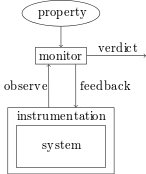
\includegraphics{resources/Runtime_Verification_Monitor.png}
\end{center}
The property is specified using some formal language. This monitor is then used to observe the system and test the specification at specific moments during execution. These points during executions can be defined within the monitor. For example when a variable is written or before a function is called. The system must sent events to the monitor so that it knows when to act and test the specification. The monitor can then report feedback to the system. The major drawback of using runtime verification is the overhead it creates. This overhead is dependent on the type of property that is checked and how many times during execution. \\
Runtime verification on smart contracts is different from general purpose languages since race conditions and deadlocks can not occur in the EVM because there is no multi threading. However other properties of runtime verification could be useful. For example monitors can observe the behaviour of a smart contract and when a property fails to satisfy the monitor could revert the transaction completely. This could help developers write more secure smart contracts. The EVM has some limitations because smart contracts are executed by every node. For example the extra computations cost extra gas, which makes the same functionality cost more Ether. Some of these limitations could be solved by checking some properties offline. Each transaction is public, which means that a specific 'Runtime Verification' node could check the properties where the normal node just execute the code without executing the monitor.

\section{Related Work}
\label{sec:RelatedWork}
There is a lot of work related to this topic. Ethereum is not the only blockchain platform that supports the deployment of smart contracts, but this section will focus on the development and research for the Ethereum blockchain specifically. There are papers discussing the verification of smart contracts. They can be further categorized as static analysis or formal verification. Additionally other contract languages have been proposed to help writing secure smart contracts. The last subsection discusses some other related work.

\subsection{Smart Contract Verification}
Due to the recent exploits that were found on the Ethereum blockchain this research area has seen a lot of attention. Especially in the field of formal verification. There are many proposals of verification tools that will help to write secure smart contracts. The security of smart contracts is important because if the bytecode of a contract is committed to the blockchain it cannot be changed afterwards. This means that testing and verification of the code before committing it to the network is important. The efforts can be categorized in two groups; static analysis and formal verification. The first class are tools that analyse the EVM code or a higher level code and check for patterns. Patterns that are known to be vulnerable get reported. The code is not actually executed, only symbolically. The second group is formal verification. These tools work by giving a specification for a given program. The tool then proves that the program is correct for all possible inputs with respect to the given specification. Some tools fully automate this process, some work with a proof assistant. Note that the Solidity code is usually translated to EVM or some intermediate language in which the proofs can be more easily automated.
\subsubsection{Static Analysis Tools}
There are many tools that are defined in this area. Most of the tools have the same functionality. You can analyse contracts using the Solidity Code or EVM bytecode. These contracts can be analysed locally or from an online provider (Ethereum mainnet or one of the test nets). Examples of such tools are Mythril \cite{mythrilrepo}, Securify \cite{securifywebsite} and Oyente \cite{luu2016making}. The Oyente tool also offers the possibility to analyse all the contracts on the whole blockchain. Their tool is not only available on Github but also has a paper which describes the choices made fo the analysis tool. The tools under this category do not test for errors in business logic. For example if a function returns too much ether on a specific input, this will not be detected by static analysis tools. 
\subsubsection{Formal Verification Tools}
To verify a contract a specification has to be written. Specification gives meaning to what the contract should do. However because Solidity is not fit for this most tools are defined at the EVM bytecode level, or introduce an intermediate contract language. These programs are then proven correct considering all possible inputs with respect to the given specification. KEVM \cite{hildenbrandt2017kevm}, a formalization of the EVM in F* \cite{grishchenko2018semantic} and eth-isabelle \cite{hirai2017defining} are very similar. All three tools are able to execute a large set of the official ethereum test suite and are able to proof specifications correct for certain contracts. Other approaches use an intermediate language over which properties can be proven correct. Lolisa \cite{yang2018lolisa} and Scilla \cite{sergey2018scilla} fall under this category. 

\subsection{Smart Contract Languages}
Smart contracts are usually written in a high level language that compiles to EVM (Ethereum Virtual Machine) bytecode. Currently the best known and most used language is Solidity (as described in detail in section \ref{sec:solidity}). But there are other options available that also compile to EVM bytecode. They differ in their syntax and influences by other languages.  
\subsubsection{Bamboo}
Bamboo is a morphing smart contract language. State transitions are a core part of the language design. This makes the state transitions in smart contracts explicit. This way it avoids re-entrancy by default. Each function is declared within a state and executing a function causes a state transition. This way there should be less surprises in the execution of smart contracts. The project is located in a repository located at \url{https://github.com/pirapira/bamboo}. As an example the smart contract for a crowd funding is used. The crowd funding usually has several stages in which different things can happen. In Solidity these stages are usually modeled using boolean variables and enforced using \texttt{modifiers}. With this approach it is hard to keep track which functions are enabled at which state. In Bamboo this is not the case since functions are declared within a state and functions modify the signature of the smart contract. 
\subsubsection{Vyper}
Vyper is a new and experimental smart contract programming language. It is maintained by the Ethereum Foundation at \url{https://github.com/ethereum/vyper}. The idea is to limit certain functions and aspects that are possible in Solidity to make writing smart contracts less error prone. It also tries to make smart contracts more human readable to make it simpler to see what will happen when a function is called. For example \texttt{modifiers}, inline assembly and class inheritance is not allowed in Vyper as opposed to Solidity. 

\subsection{Other related work}
A number of other proposals have been published which try to make smart contracts more secure. They do not belong to a certain category but are related to the current work. Some projects only have source code available and do not have documentation or a paper.
\subsubsection{ContractLARVA}
ContractLARVA can be found on github at \url{https://github.com/gordonpace/contractLarva}. Following the instructions on the README you can write a specification and a contract in Solidity. The compiler will combine these two and output a new Solidity contract with the runtime verification checks in place. Properties have to be specified using \textit{dynamic event automata} (DEA) \cite{CGG08FMICS}. The tool is based on a similar tool called LARVA for Java. \\
For example consider the following Solidity contract. In this contract we would like to monitor the variable \texttt{number}, it should always be positive.
\lstinputlisting[language=Solidity]{examples/MyContract.sol}
The monitor has to be defined in DEA syntax.
\lstinputlisting[language=C]{examples/MyDEA.dea}
The specification and contract are combined into a new contract with the added behaviour. The output of the tool can be seen below.
\lstinputlisting[language=Solidity]{examples/MyContractOutput.sol}
The above example is a contract that can be deployed to a local testnet. However all calls to the function \texttt{setNumber} will fail because the code is not initialized correctly. The \texttt{LARVA\_Status} is never set to running thus the modifier \texttt{LARVA\_ContractIsEnabled} will throw an exception. This approach has several limitations, for example monitors can only be added with states. Even if the contract does not represent a state machine. The states are represented as \texttt{int8} in the generated contract code, which cost extra gas. States have to be initialized in the beginning. This means that the generated contract has to have a constructor and potentially call the original constructor. This changes the contract interface and thus could limit the testing of the contract because other applications could depend on it. To test a certain specification on previous values the variable is stored to a storage location. This causes a lot of extra gas cost where should be possible to store in in \texttt{memory}. In the previous example see the variable \texttt{LARVA\_previous\_number}.

\subsubsection{Ethereuem-runtime-verification}
This project is located at \url{https://github.com/shaunazzopardi/ethereuem-runtime-verification}. No documentation is available for this project. It mentions the LARVA project in the description in that it differs from LARVA because this runtime-verification tool can dynamically add properties to an already deployed smart contract.

\subsubsection{The Hydra Project}
The Hydra Framework is a project for smart contracts on the Ethereum network. It tries to make smart contracts more secure by making multiple implementations of the same contract. They call this \textit{N-of-N-version programming}. The different implementations are controlled by a meta contract which forwards the incoming calls to all the implementations. If the implementations do not agree on a single answer, the meta contract will be able to react on this. When such a vulnerability is found a bounty is given to the person who exploited the vulnerability. They call this principle \textit{the exploit gap}, this means that a hacker should claim the bounty instead of exploiting the vulnerability. More information can be found in their paper \cite{breidenbachenter}. 

\subsubsection{FSolidM}
FSolidM \cite{mavridou2018tool} is a fully functional tool which helps developing secure smart contracts. It provides a GUI to specify contracts using finite state machines (FSM). These FSMs are then translated to secure solidity contract code. This tool helps creating secure smart contracts since the semantics of the FSM is well defined. The tool comes with a code generator for generating Solidity code, and also the possibility to define plugins. These plugins can be used to define certain patterns that implement common design patterns or include security constraints. 
\subsubsection{Quantitative Analysis of Smart Contracts}
Chatterjee et al. \cite{chatterjee2018quantitative} analyse the utility (expected payout) for smart contracts. It does so by using game theory and incentives to analyse a stateful game. It uses a simplified contract language and translates these contracts to state-based games. These games can then be analysed by the tool for their expected payout. The functions in the games are assumed to be executed at distinct timeslots. This is however not the case for Ethereum since one can always write a specific contract to call all functions within the same transaction. Also calls to other contracts are not considered while this is where most of the complexity and vulnerabilities are discovered in real world contracts.


\section{Final Project}
This document serves as a starting point for the Final Project. This paper describes the requirements and related work of a concept tool that is to be developed in the Final Project. The tool will make it possible to write specifications at the same level of Solidity code. These specifications will then be parsed and can be used for a number of different analyses. For example they can be added as extra checks in the code, which is called runtime verification. Writing the specification at the level of Solidity code helps understanding the problem. It can also be used to generate code that other tools can use for formal verification as mentioned in Section \ref{sec:RelatedWork}. \\
The result of this are a research questions that will be answered during the development of the tool in the Final Project. The project can be seen in three different steps that have to be taken.
\begin{enumerate}
    \item \textbf{Property specification/definition.}
    The first step is to decide and analyse which properties should be able to be checked and specified. Properties should make sense and should be able to be checked within Solidity. This raises the question:
    \textit{What properties should the tool be able to identify and specify?}. Specifically the \textit{syntax} has to be defined. And a \textit{parser} has to be written to decide if properties are according to the defined syntax. 
    \item \textbf{Tool development.}
    The next step is defining the output of the tool. In other words: \textit{What can be generated from the specification and smart contract source code?} For example some properties can be checked using static analysis and some have to be implemented in Solidity. The properties that are inserted into the Solidity code are checked at runtime. Another possibility is to generate code for different formal verification tools which are described in Section \ref{sec:RelatedWork}.
    \item \textbf{Tool usage on smart contract.}
    The last step is to test the tool on real world smart contract. And see if it can detect vulnerabilities that would otherwise have not been found. \textit{How can the tool be used to detect vulnerabilities in smart contracts?}.
\end{enumerate}

\subsection{Tasks and Planning}
To answer each question different steps have to be taken. For the planning see the diagram below. 
\begin{enumerate}
    \item Property specification 
    \begin{enumerate}[label*=\arabic*.] 
        \item Decide on technique/tool. There are multiple options to implement a parser. One of the solutions is to extend the Solidity compiler which is open source on Github \footnote{https://github.com/ethereum/solidity}. Another solution is to use the ANTLR based grammar which is kept up to date independently \footnote{https://github.com/solidityj/solidity-antlr4}. 
        \item Extend Grammar. The grammar has to be extended to accept the specifications that should be inserted into the contracts. It should be able to parse the extended annotations.
        \item Design. Design the architecture for the parser and validator. The parser can be generated from the grammar automatically. But the specification has to be validated. For example the identifiers that are used must be present in the contract and only for all constructs can be used on arrays.
        \item Implementation. Implement the property specification and syntax validation in the technique that was chosen in task 1.
    \end{enumerate}
    \item Tool output 
    \begin{enumerate}[label*=\arabic*.] 
        \item Design. Output of the previous step is a parsed and valid specification. Next step is generate the runtime verification code. First we need to decide how to implement this functionality.
        \item Implementation.
    \end{enumerate}
    \item Tool Analysis 
    \begin{enumerate}[label*=\arabic*.] 
        \item Examples. To test the tool examples of smart contracts are needed. These should then be annotated with additional properties and then be passed on through the tool. 
        \item Gas Analysis. One thing to analyse is the extra gas usage the extra checks use and compare it to the gas cost of the base contract.
        \item Other analysis tools. Other analysis can be done with the specifications. A few of them are mentioned during the introduction, but they could be used to generate code that can be used for a formal verification tool. This means that the solution must be easily extensible.
    \end{enumerate}
    \item Project 
    \begin{enumerate}[label*=\arabic*.] 
        \item Report. The report should be updated throughout the project. If a certain task is completed the report should be updated as well. 
        \item Final Presentation. 
    \end{enumerate}
\end{enumerate}
    
\begin{center}
    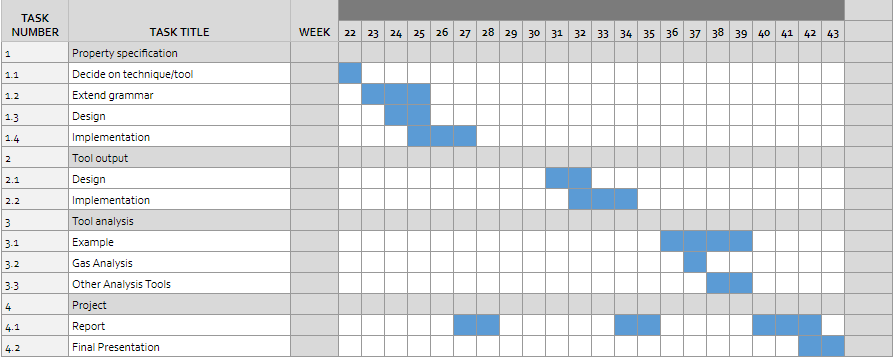
\includegraphics[angle =90]{resources/Planning.png}
\end{center}


\bibliographystyle{IEEEtran}
\bibliography{IEEEfull,references}
\end{document}